\chapter{Le projet Yuukou 2}

\section{Recherches}

\subsection{Architecture du projet}
\label{section:architectureProjet}

Le premier travail a \'et\'e la r\'eflexion sur comment mettre en place une solution pouvant communiquer avec Nagios dont une description sera faite au \S~\ref{section:nagios}.
Les figures~\ref{figure:architectureProjetServiceWeb} et~\ref{figure:architectureProjetAffichage} pr\'esentent le fruit des recherches qui ont \'et\'e faites sur la mise en place du projet \YuukouII.

\begin{figure}[!ht]
	\centering
	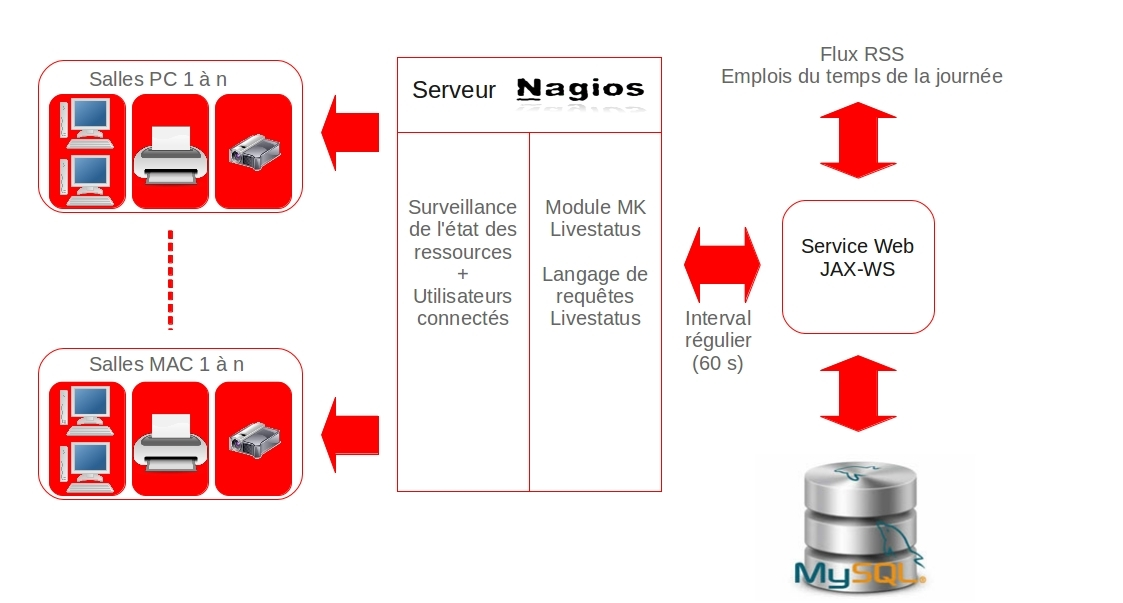
\includegraphics[scale=0.35]{architectureProjetServiceWeb.jpg}
	\caption{Architecture du projet, partie service Web}
	\label{figure:architectureProjetServiceWeb}

\end{figure}

\begin{figure}[!ht]
	\centering
	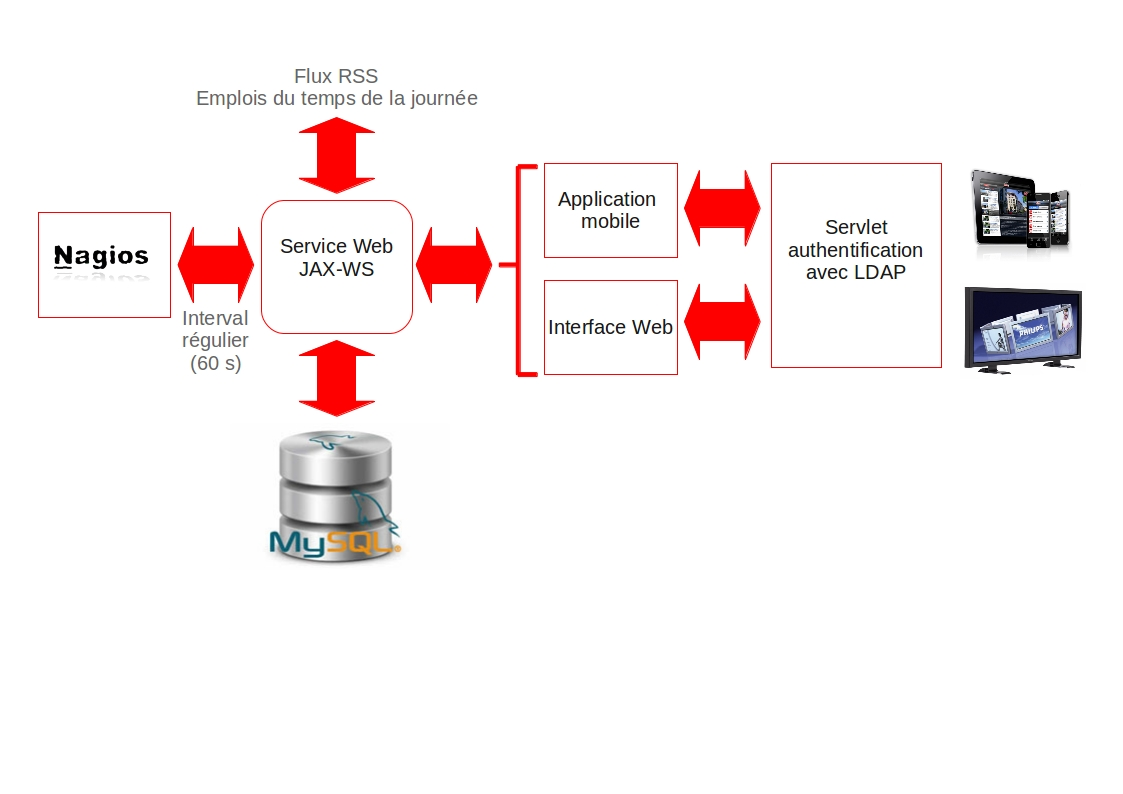
\includegraphics[scale=0.35]{architectureProjetAffichage.jpg}
	\caption{Architecture du projet, partie affichage}
	\label{figure:architectureProjetAffichage}

\end{figure}

\subsubsection{Partie service Web}

Basiquement Nagios sert \`a surveiller les ressources auxquelles il lui est permis d'acc\'eder.
De ce fait, il doit garder des traces des informations qu'il r\'ecup\`ere.
Ces informations sont stock\'ees dans un fichier.
C'est pourquoi un module existe sp\'ecialement pour acc\'eder aux informations contenu dans ce fichier. 
Le module \textit{MK Livestatus} permet \`a l'aide d'un langage de requ\^etes qui lui est propre, de r\'ecup\'erer les informations que garde Nagios.

Le service Web doit permettre, dans un premier temps, de r\'ecup\'erer toutes les informations utiles pour un archivage des donn\'ees.
Elles sont stock\'ees dans une base de donn\'ees MySQL.
\noindent Ces informations sont :

\begin{itemize}
	\item les donn\'ees r\'ecup\'er\'ees via le module \textit{MK Livestatus}, la r\'ecup\'eration doit \^etre faite \`a intervalles r\'eguliers;
	\item les diff\'erents emplois du temps de toutes les salles que Nagios surveille, la r\'ecup\'eration doit \^etre faite une fois par jour;
	\item les donn\'ees sur un utilisateur inconnu (nom, pr\'enom, r\^ole : \'etudiant par exemple, photo) via un serveur LDAP.

\end{itemize}

\subsubsection{Partie affichage}

Dans un deuxi\`eme temps, le service Web doit pouvoir retourner ces informations tri\'ees \`a un utilisateur normal ou un administrateur afin de garantir l'affichage sous la forme d'une application mobile ou d'une interface Web.
La r\'eflexion doit ainsi se porter sur le contenu des diff\'erentes m\'ethodes auxquelles un utilisateur pourra avoir acc\`es (en fonction qu'il soit administrateur ou non).
Le but \'etant un affichage le plus rapide possible des informations demand\'ees.

L'utilisateur doit s'authentifier via un Servlet$^*$ qui communique avec LDAP$^*$ et qui donne un acc\`es \`a l'application.
Le reste de la communication est s\'ecuris\'ee comme expliqu\'e dans le \S~\ref{section:securisation}.

Le dernier point est de choisir un format pour les donn\'ees qui seront \'echang\'ees entre le service Web et l'application cliente.

C'est sur cette partie que Yacine MAGHEZZI est intervenu durant son stage.

\subsection{Nagios}
\label{section:nagios}

\begin{figure}[!ht]
	\centering
	
\includegraphics[scale=0.5]{nagiosLogo.jpg}
	\caption{Logo de Nagios}

\end{figure}

\subsubsection{Pr\'esentation}

Nagios est une application permettant la surveillance syst\`eme et r\'eseau de toute une infrastructure informatique.
Nagios compl\`ete cette surveillance en offrant la possibilit\'e d'alerter les \'equipe en charge de l'infrastructure en cas d'apparition de probl\`emes comme une panne ou encore un fonctionnement anormal.
C'est actuellement la solution de surveillance la plus efficace du march\'e.

\parpic{
	\begin{minipage}{0.20\textwidth}
		
\includegraphics[scale=0.6]{netsaintLogo.jpg}
	\end{minipage}}
Nagios a \'et\'e cr\'e\'e en 1999 et portait initialement le nom de \textit{NetSaint Network Monitor}.
Il est \'ecrit en C et est con\c{c}u pour un environnement Unix.
Le projet a \'et\'e maintenu jusqu'en 2002 avant de changer de nom pour devenir Nagios en r\'eponse \`a une contestation judiciaire par les propri\'etaires d'une marque similaire.
N.A.G.I.O.S. est l'acronyme r\'ecursif de \og{}\textit{Nagios Ain't Gonna Insist On Sainthood}\fg{} o\`u Sainthood est une r\'ef\'erence \`a \textit{NetSaint}.

Maintenant connu sous le nom de Nagios XI, Nagios est un logiciel libre sous la licence GNU GPL V2. 
Il est disponible sur son site Internet\cite{biblio:siteNagios} en version 3.2.1.

\subsubsection{Fonctionnement}

\noindent L'architecture de base de Nagios est tr\'es simple, elle comporte :

\begin{itemize}
	\item un ordonnanceur pour g\'erer les v\'erification ainsi que les actions \`a prendre sur les diff\'erents incidents;
	\item une partie graphique : visible \`a travers un simple serveur Web;
	\item des sondes : greffons (ou \textit{plugins} en anglais) dans Nagios, ce sont de petits \textit{scripts} permettant d'effectuer diverses v\'erifications.

\end{itemize}

\vspace{0.20cm}

\`A la base, Nagios est un moteur d'ordonnancement de v\'erifications diverses et vari\'ees dont les v\'erifications sont effectu\'ees via des greffons.
Ces v\'erifications peuvent \^etre la charge d'utilisation du CPU\protect\footnote{\textit{Central Processing Unit} ou processeur en fran\c{c}ais}, l'espace disque utilis\'e ou encore qui est connect\'e actuellement.
Dans le cadre de la v\'erification de l'infrastructure, deux types de machines sont observ\'ees : les ordinateurs dot\'es de Windows et les ordinateurs dot\'es de Macintosh.

Nagios \'etant install\'e et fonctionnel depuis un peu plus d'un an sur le site de New Cavendish, les greffons pour observer les deux types de machines ont d\'ej\`a \'et\'e d\'evelopp\'es.
Pour les machines fonctionnant sous Windows, le greffon est en fait l'appel \`a la commande Unix \textit{Winexe} qui permet l'ex\'ecution de commandes \`a distance sur des machines Windows.
Pour les machines fonctionnant sous Macintosh, le greffon effectue une connexion SSH\protect\footnote{\textit{SecureShell}}, offrant une connexion s\'ecuris\'ee sur une machine distante pour ensuite ex\'ecuter la commande Unix \textit{who} permettant l'obtention de l'utilisateur connect\'e.
Pour les machines b\'en\'eficiant d'un double \textit{boot} (d'un d\'emarrage de l'ordinateur permettant de choisir entre deux syst\`emes d'exploitation) Windows-Unix, seul le syst\`eme Windows est surveill\'e.
La configuration actuelle de Nagios ne permet pas de r\'ecup\'erer avec exactitude l'utilisateur connect\'e sur le syst\`eme Unix.
Il est juste possible de savoir que l'ordinateur est occup\'e, mais pas par qui.

La configuration de Nagios s'articule entre diff\'erents concepts : les \textit{hosts}, les \textit{hostgroups} les \textit{services}.
Un \textit{host} repr\'esente un ordinateur, cet ordinateur poss\`ede des \textit{services} comme le service \textsf{check\_whoisloggedin} permettant de savoir si un utilisateur est actuellement connect\'e sur ladite machine.
Il faut enfin partie d'un groupe d'ordinateurs \textit{hostgroups} qui repr\'esente une salle informatique au sein de l'universit\'e.

\subsubsection{\og{}Monitoring\fg{} \`a l'universit\'e}

Initialement, Nagios surveillait juste les machines se situant sur le campus de New Cavendish, soit 31 salles PC seulement machines.
Actuellement, ce sont 102 salles qui sont sous la surveillance de Nagios, soit 99 salles utilisant Windows soit 1920 PC, 3 salles utilisant des Macintosh soit 63 MAC, pour un total de 1983 machines \`a travers toute l'universit\'e : la grande majorit\'e des ordinateurs de l'universit\'e.
Il faut noter que seuls les Macintosh de New Cavendish sont sous surveillance, les autres n\'ecessitant d'\^etre list\'es et des acc\`es diff\'erents.
De ce fait, le nombre de machines devrait augmenter par la suite.

\subsubsection{Vue sur la surveillance de Nagios}

Les figures~\ref{figure:nagiosGeneral} et~\ref{figure:nagiosCG24}  donnent un aper\c{c}u de l'interface graphique de configuration mais aussi de suivi de Nagios.
La figure~\ref{figure:nagiosGeneral} offre une vue d'ensemble sur tous les  \textit{hosts} de tous les \textit{hostgroups} surveill\'es.
La figure~\ref{figure:nagiosCG24}, quant \`a elle, offre une vue pour un \textit{hostgroup} sp\'ecifique : la salle pourtant le nom \textsf{e-cg24}.

\begin{figure}[!ht]
	\centering
	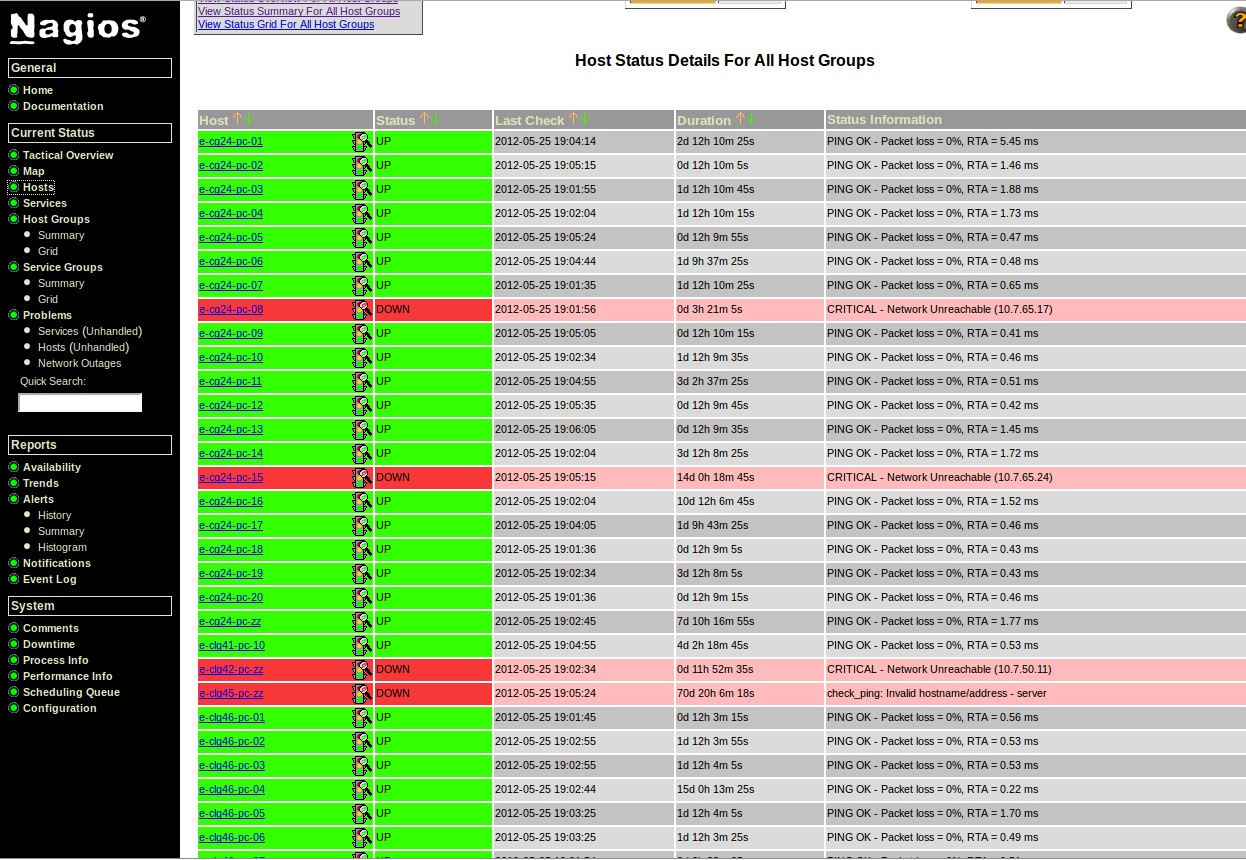
\includegraphics[scale=0.35]{nagiosGeneral.jpg}
	\caption{Exemple d'affichage de Nagios, vue sur tous les \textit{hostgroups}}
	\label{figure:nagiosGeneral}
	
\end{figure}

\begin{figure}[!ht]
	\centering
	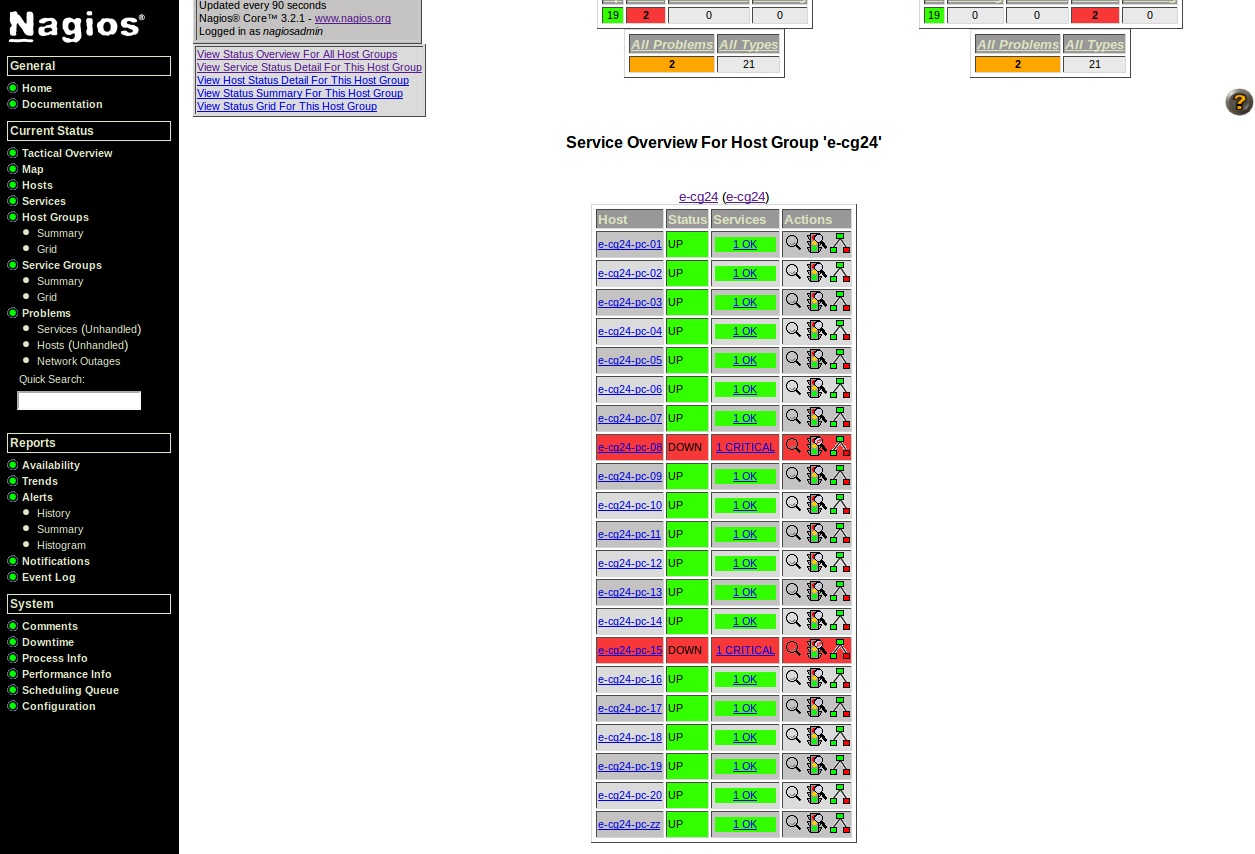
\includegraphics[scale=0.35]{nagiosCG24.jpg}
	\caption{Exemple d'affichage de Nagios, vue sur tous les \textit{hosts} d'un \textit{hostgroup} sp\'ecifique}
	\label{figure:nagiosCG24}
	
\end{figure}




TODO REPRENDRE

\subsection{L'IDE NetBeans}
\label{section:netbeans}

\begin{figure}[!ht]
	\centering
	
\includegraphics[scale=0.25]{netbeansLogo.jpg}
	\caption{Logo de NetBeans}

\end{figure}

NetBeans est un IDE\protect\footnote{\textit{Integrated Development Environment}}$^*$ \textit{open source} d\'evelopp\'e par Sun Microsystems permettant le d\'eveloppement en utilisant les langages de programmation tels que Java, JavaScript, PHP$^*$, C, C++, et autres.
Il est \'ecrit en Java et fonctionne sous Windows, Mac OS, Linux, Solaris et d'autres plates-formes du moment qu'elles poss\`edent une JVM\protect\footnote{\textit{Java Virtual Machine}}$^*$ compatible.

NetBeans permet de d\'evelopper et d\'eployer rapidement des applications graphiques Swing, des Applets, des JSP/Servlets et des architectures J2EE\protect\footnote{\textit{Java Platform, Enterprise Edition}}.
Il poss\`ede toutes les fonctionnalit\'es recherch\'ees dans un IDE$^*$ moderne (coloration syntaxique, refactoring, d\'ebogueur, \ldots) et ajoute, dans le cas d'un d\'eveloppement d'un service Web comme pour ce projet, un support avec la derni\'ere version de GlassFish, permettant notamment de faire des \og{}deploy on save\fg{}, de d\'eployer les applications Web sur un serveur distant et de contr\^oler le serveur (suivre la sortie de logs, d\'emarrer, arr\^eter le serveur). 
Il donne acc\`es \`a une gestion simple du serveur d'application GlassFish qui sera utilis\'e dans le projet.
Sa premi\`ere version date de 1996 et portait le nom Xelfi. 
Il est disponible sur son site Internet\cite{biblio:siteNetbeans} en version 7.1.2.

\subsection{Le serveur Web GlassFish}
\label{section:glassfish}

\begin{figure}[!ht]
	\centering
	
\includegraphics[scale=0.35]{glassfishLogo.jpg}
	\caption{Logo de GlassFish}

\end{figure}

GlassFish est un serveur d'application \textit{open source} d\'evelopp\'e par Sun Microsystems pour les plates-formes Java EE\protect\footnote{\textit{Java Platform, Entreprise Edition}} 5 et 6, et est maintenant maintenu par Oracle Corporation.
Il dispose de nombreux outils pour faciliter le d\'eveloppement, le d\'eploiement et la maintenance d'application.
Un de ses avantages est qu'il est particuli\`erement bien int\'egr\'e \`a NetBeans, ce qui permet un d\'eploiement tr\`es rapide des applications ainsi qu'une trace d'ex\'ecution lors du fonctionnement.
GlassFish est disponible sur son site Internet\cite{biblio:siteGlassfish} en version 3.1.2.

\subsection{Le SGBD MySQL}

Un des objectifs du projet {\YuukouII} est un archivage temporel des donn\'ees.
Le but \'etant de g\'en\'erer des statistiques d'utilisation des salles informatiques des diff\'erents campus par exemple.

\begin{figure}[!ht]
	\centering
	
\includegraphics[scale=0.75]{mysqlLogo.jpg}
	\caption{Logo de MySQL}
	
\end{figure}

MySQL est le Syst\`eme de Gestion de Base de Donn'ees (SGBD) la plus populaire qui fonctionne comme un serveur fournissant un acc\`es multi-utilisateurs \`a des bases de donn\'ees de type SQL$^*$.
Il a \'et\'e cr\'e\'e par MySQL AB en 1995, rachet\'e par Sun Microsystems et est maintenant maintenu par Oracle.
Il pr\'esente les avantages d'\^etre \textit{open source}, gratuit, fiable, rapide et facile \`a utiliser.
Il est tr\`es souvent utilis\'e avec le langage de cr\'eation de pages Web dynamique PHP$^*$.
C'est donc avec cet outil que les donn\'ees de {\YuukouII} seront archiv\'ees.
MySQL est disponible sur son site Internet\cite{biblio:siteMySQL} en version 5.5.24.



\section{Communication avec Nagios}

Nagios offre la surveillance d'un grand ensemble de machines dans l'universit\'e. 
Cependant s'il n'y a aucune mani\`ere de r\'ecup\'erer ces informations, il n'aurait aucune utilit\'e dans le projet.
Ainsi un module a \'et\'e d\'evelopp\'e, son but \'etant de pouvoir interroger Nagios et obtenir ses r\'eponses le plus rapidement et simplement possible.

\subsection{Le module MKLivestatus}
\label{section:moduleMKLivestatus}

Le module MKLivestatus permet un acc\`es imm\'ediat au statut de Nagios ainsi qu'\`a ses donn\'ees de logs.
Avant le module, une fa\c{c}on classique de r\'ecup\'erer les informations importantes \'etait de \textit{parser} le fichier \textsf{status.dat}, qui est cr\'e\'e automatique par Nagios \`a chacun de ses cycles.
Ce fichier contient toutes les informations concernant les services et les machines que Nagios surveille.
\textit{Parser} ce fichier s'av\`ere d\'elicat, surtout pour extaire quelques informations.
Il existe bien une mani\`ere alternative de r\'ecup\'erer ces informations avec le module NDO.
Ce module est directement charg\'e dans le processus de Nagios et \`a chaque nouveau cycle, il envoie les mises \`a jour via une socket UNIX$^*$ \`a un processus auxiliaire qui se charge de mettre \`a jour une base de donn\'ees.

Les avantages \'etant une mise \`a jour imm\'ediate de l'information et une simplicit\'e et rapidit\'e d'acc\`es aux bases de donn\'ees pour les applications.
Mais d'un autre cot\'e, la mise en place de ce syst\^eme est complexe, elle n\'ecessite une administration humaine de la base de donn\'ees, la consommation CPU est significative juste pour garder la base \`a jour et son entretien r\'egulier peut bloquer Nagios pendant un moment (cela d\'epend de la taille de l'infrastructure).

Le module MKLivestatus reprend le principe de NDO dans l'int\'egration directe dans le processus Nagios, cependant, la diff\'erence de taille est qu'il ouvre juste une socket de communication par laquelle les donn\'ees peuvent \^etre retrouv\'ee \`a la demande.
La socket ouverte par d\'efaut par MKLivestatus est une socket UNIX$^*$, mais il est possible de configurer une socket Internet classique sur un port choisi et accessible seulement par certaines machines.
Par cette socket, il est possible d'envoyer une requ\^ete vers une cible sp\'ecifique comme un service, une machine, un ensemble de machines, \ldots{}
La r\'eponse est imm\'ediate et les donn\'ees renvoy\'ees ont \'et\'e directement lu dans les structures de donn\'ees internes de Nagios.

\noindent MKLivestatus offre donc de nombreux avantages :

\begin{itemize}
	\item consommation CPU non mesurable, juste une petite consommation lors de l'ex\'ecution d'une requ\^ete;
	\item pas d'ecritures sur le disque;
	\item acc\`es aux donn\'ees beaucoup plus rapide qu'avec un \textit{parsing} du fichier \textsf{status.dat} ou l'ex\'ecution de requ\^etes SQL$^*$.
	\item pas de configuration, d'administration ou autre, tout est install\'e automatiquement.

\end{itemize}

\vspace{0.20cm}

MKLivestatus est disponible sur le site Internet\cite{biblio:siteMklivestatus} de Mathias Kettner en version stable 1.1.12p7.

\subsection{Requ\^etes pour Nagios}

\subsubsection{\'Ecriture des requ\^etes avec LQL}

LQL, Livestatus Query Language, prononc\'e \og Liquel\fg, est un langage sp\'ecialement con\c{c}u pour communiquer avec le module MKLivestatus via une socket.
Il ressemble un peu au langage SQL$^*$.

\noindent Chaque requ\^ete consiste en :

\begin{itemize}
	\item une commande commen\c{c}ant par le mot cl\'e \textsf{GET} suivit du nom de la \textit{table};
	\item un nombre arbitraire de lignes d'en-t\^ete consistant en un mot cl\'e, un double-point et une liste d'arguments;
	\item une ligne vide ou une fin de transmission (pour fermer la proc\'edure d'envoi sur la socket).

\end{itemize}

\vspace{0.20cm}

Tous les mots cl\'es sont sensibles \`a la casse. 
La version actuelle de Livestatus donne acc\`es \`a seize tables dont voici les principales :

\begin{itemize}
	\item \textbf{hosts} : les h\^otes surveill\'es par Nagios;
	\item \textbf{services} : les services de Nagios, reli\'es avec toutes les donn\'ees de la table \textit{hosts};
	\item \textbf{hostgroups} : les groupes d'h\^otes cr\'e\'es dans Nagios;
	\item \textbf{servicegroups} : les groupes de services cr\'e\'es dans Nagios.

\end{itemize}

\vspace{0.20cm}

Les requ\^etes peuvent aussi \^etre affin\'ees avec la s\'election de certaines colonnes, la cr\'eation de filtres sur les r\'esultats (tous les r\'esultats dont la valeur est \'egale \`a deux), compter des r\'esultats, faire des comparaisons avec des expressions r\'eguli\`eres, \ldots{}
Au final, LQL s'av\`ere tr\`es flexible d'utilisation.
La figure~\ref{code:exempleLQL} donne un exemple de requ\^ete permettant de r\'ecup\'erer tous les services avec leur \'etat actuel \`a 2.

\vspace{0.20cm}

\begin{figure}[!ht]
	\lstinputlisting[language=LQL]{codes/nagiosExemple.ngs}
	%\captionof{figure}{Exemple de requ\^ete LQL}
	\caption{Exemple de requ\^ete LQL}
	\label{code:exempleLQL}

\end{figure}

Les \textit{scripts} Nagios utilis\'es tout au long du stage sont disponibles en annexe~\ref{chapterAnnexe:fichiersLQLNagios} de ce rapport.

\subsubsection{Ex\'ecution des requ\^etes}

Comme pour une base de donn\'ees SQL$^*$, toutes les tables poss\`edent un nombre de colonnes.
Si une requ\^ete est pass\'ee sans param\^etres, toutes les colonnes seront retourn\'ees dans l'ordre alphab\'etique.

Comme vu dans au \S~\ref{section:moduleMKLivestatus}, il existe deux mani\`eres d'acc\'eder \`a la socket de MKLivestatus.
La premi\`ere m\'ethode est avec une socket UNIX$^*$. 
Pour ce faire, MKLivestatus fournit pendant son installation un petit utilitaire appel\'e \textsf{unixcat} permettant de communiquer avec une socket UNIX$^*$.
Sous forme d'une commande shell, cet utilitaire envoit toutes les donn\'ees lu par l'entr\'ee standard (stdin) \`a la socket et \'ecrit sur la sortie standard (stdout) tout ce qu'il re\c{c}oit de la socket.
Voici un exemple d'ex\'ecution en utilisant la commande \textsf{unixcat} : 

\begin{center}
	\textsf{echo 'GET hosts' | unixcat /var/lib/nagios/rw/live}.

\end{center}

La seconde mani\`ere consiste en l'ouverture d'une socket Internet sur un port pr\'ed\'efini.
Avec cela, il est possible d'acc\`eder depuis le r\'eseau de l'universit\'e au serveur h\'ebergeant Nagios.
Il suffit ensuite d'envoyer via la commande UNIX \textsf{netcat}, qui permet d'ouvrir des sockets serveurs et clientes, un fichier contenant la requ\^ete LQL :

\begin{center}
	\textsf{cat requete | netcat yuukou-ws.wmin.ac.uk 6557}.

\end{center}

Dans le cadre du projet, l'utilisation d'une socket UNIX$^*$ en Java n\'ecessite l'installation de biblioth\`eques de type JNI\protect\footnote{\textit{Java Native Interface}}.
Ce sont en fait des biblioth\`eques qui permettent l'int\'egration du code \'ecrit en Java avec du code \'ecrit dans un autre langage tel le C ou le C++.
Cette installation est plus ou moins complexe et n\'ecessite une certaine configuration du serveur, ainsi, il est plus simple d'ouvrir une socket Internet plut\^ot que d'essayer la configuration d'une socket UNIX$^*$ avec JNI.
De plus, au point de vue rapidit\'e, l'avantage de MKLivestatus est d'\^etre directement int\'egr\'e dans Nagios, de ce fait, les requ\^etes sont trait\'ees imm\'ediatement.

Le tableau~\ref{table:comparatifTemps} montre un comparitif des temps d'ex\'ecution mesur\'es avec la commande UNIX \textsf{time} pour 100 requ\^etes.
La requ\^ete de la figure~\ref{annexe:nagiosGetResources} se trouvant en annexe~\ref{chapterAnnexe:fichiersLQLNagios} de ce rapport a \'et\'e utilis\'ee pour effectuer ces tests.
Chaque r\'eponse contient 1983 lignes.

\begin{table}[!ht]
	\centering
	\begin{tabular}{|>{\columncolor{grisclair}}c|c|c|}
		\hline
		\rowcolor{grisclair} \textbf{time} & \textbf{unixcat} & \textbf{netcat}\\
		\hline
		R\'eel & 1m44.462s & 1m42.129s\\
		\hline
		Utilisateur & 0m0.372s & 0m0.432s\\
		\hline
		Syst\`eme & 0m0.268s & 0m0.404s\\
		\hline

	\end{tabular}

	\caption{Comparatif des temps d'ex\'ecution entre la commande \textsf{netcat} et la commande \textsf{unixcat}}
	\label{table:comparatifTemps}

\end{table}

Apr\`es 100 requ\^etes, il est visible qu'utiliser une socket UNIX$^*$, pour une ex\'ecution syst\`eme est presque deux fois plus rapide que l'utilisation d'une socket Internet.
Cependant, l'application ne n\'ecessite pas l'ex\'ecution de nombreuses requ\^etes simultan\'ees.
Une seule sera effectu\'ee \`a chaque cycle comme d\'ecrit au \S~\ref{section:cyclePrincipal}.
De ce fait, l'utilisation d'une socket Internet convient dans la r\'ecup\'eration des informations de Nagios.

\subsubsection{R\'ecup\'eration de l'information}

Suite \`a l'ex\'ecution de la requ\^ete, l'information est retourn\'ee par Nagios, elle est ensuite \textit{pars\'ee} en fonction du type de la requ\^ete et les informations sont trait\'ees.
Nagios retourne les informations sous une forme bien sp\'ecifiques : 

\begin{itemize}
	\item une ligne correspond \`a une ligne de la table demand\'ee;
	\item la ligne contient toutes les colonnes de la table ou seulement celles demand\'ees dans la requ\^ete.
	Chaque colonne est s\'epar\'ee d'une autre par un \textsf{; (point-virgule)}.

\end{itemize}

\vspace{0.20cm}

Des exemples de r\'eponses correspondant aux requ\^etes de l'annexe~\ref{chapterAnnexe:fichiersLQLNagios} sont disponibles dans l'annexe~\ref{chapterAnnexe:reponseLQLNagios}.

Nagios poss\`ede sa propre fa\c{c}on de nommer une salle ou encore un ordinateur.
\noindent Les salles dans Nagios sont nomm\'ees comme suit : 

\begin{center}
	\textsf{abr\'eviation du lieu---nom de la salle}

\end{center}

\noindent Les diff\'erentes abr\'eviations sont les suivantes :

\begin{table}[!ht]
	\centering
	\begin{tabular}{|c|c|}
		\hline
		\rowcolor{grisclair} \textbf{Abr\'eviation} & \textbf{Description}\\
		\hline
		e & \textit{Electronics and Computer Science}\\
		\hline
		h & \textit{Harrow}\\
		\hline
		l & \textit{Little Tichtfield Street}\\
		\hline
		m & \textit{Marylebone}\\
		\hline
		n & \textit{New Cavendish Street}\\
		\hline
		r & \textit{Regent Street}\\
		\hline
		w & \textit{Wells Street}\\
		\hline
	
	\end{tabular}
	
	\caption{Abr\'eviations et lieux utilis\'es par Nagios pour nommer les salles et ordinateurs}
	\label{table:abreviation}

\end{table}

Ainsi, la salle \textsf{4111} se trouvant sur le campus de New Cavendish sera identifi\'ee de cette mani\`ere : \textsf{n-4111}.

\noindent Les ordinateurs sont nomm\'ees en suivant la m\^eme logique :

\begin{center}
	\textsf{abr\'eviation du lieu---nom de la salle---type ordinateur---numero ordinateur}
	
\end{center}

Le type d'ordinateur peut \^etre de deux type : \textsf{pc} si c'est un PC ou \textsf{mc} si c'est un Macintosh.
Ainsi, un ordinateur se trouvant dans la salle \textsf{n-4111}, \'etant un Macintosh et portant le num\'ero 1 sera identifi\'e comme suit : \textsf{n-4111-mc-01}.



\section{Fonctionnement du service Web}

Le service Web peut se d\'ecomposer en deux grandes parties.
La premi\`ere consiste en un cycle principal qui a pour but de r\'ecup\'erer les informations de Nagios et de les traiter.
La deuxi\`eme consiste en de multiples fonctions pouvant \^etre accessibles soit par un administrateur, soit par un utilisateur normal et permettant le retour d'une partie des informations accumul\'ees avec le cycle principal.
TODO reprendre

\subsection{Le cycle principal}
\label{section:cyclePrincipal}

C'est en quelque sorte le moteur du projet.
Il collecte des informations de Nagios, et effectue diverses op\'erations sur la base de donn\'ees pour la maintenir \`a jour.
La figure~\ref{figure:cyclePrincipal} permet de voir les diff\'erentes \'etapes qui composent le cycle principal du service Web.

\begin{figure}[!ht]
	\centering
	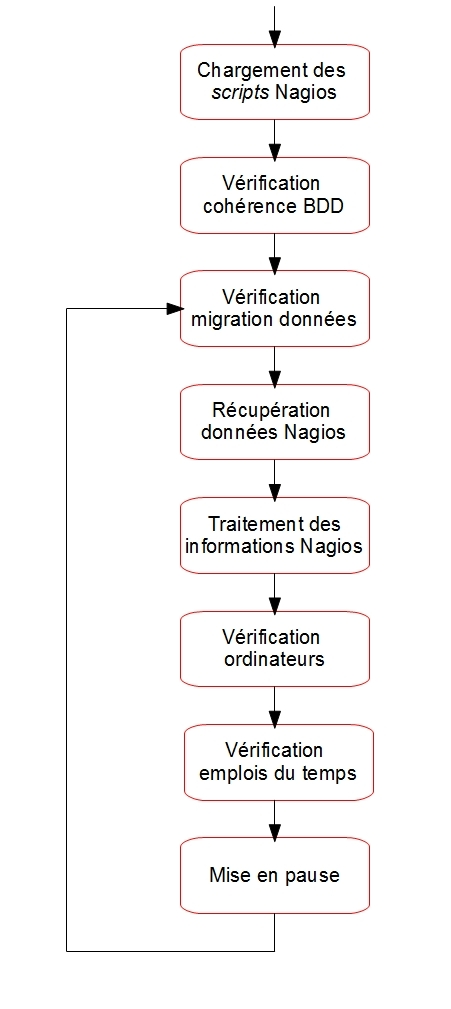
\includegraphics[scale=0.35]{cyclePrincipal.jpg}
	\caption{Sch\'ema du d\'eroulement du cycle principal du service Web}
	\label{figure:cyclePrincipal}
	
\end{figure}

Dans un premier temps, \`a la premi\`ere ex\'ecution du cycle, les diff\'erents \textit{scripts} \'ecris en LQL Nagios sont charg\'es en m\'emoire.
Ensuite, une v\'erification de la coh\'erence des donn\'ees contenues dans les tables permettant de g\'erer l'archivage des donn\'ees est effectu\'ee.
Cette v\'erification a pour but de s'assurer que il n'y a pas des donn\'ees absurdes de connexion : les donn\'ees de connexion dont dat\'ees de plus de 6 heures pour la table \textsf{yuukou\_who} et les donn\'ees de connexion dont la diff\'erence entre la date de d\'ebut de connexion et la date de fin de connexion est de plus de 6 heures elle aussi.
Si de telles donn\'ees sont trouv\'ees, elles sont automatiquement effac\'ees de la table auxquelles elles appartiennent.

L'\'etape suivante entre dans le d\'ebut du cycle \`a proprement parler.
Elle a pour objectif de v\'erifier si des donn\'ees de la table \textsf{yuukou\_last} ont besoin d'\^etre d\'eplac\'ees.
Des explications sur la migration des donn\'ees se trouvent au\S~\ref{section:migrationDonnees}.

Suite \`a cette v\'erification, les \textit{scripts} Nagios sont envoy\'es et les informations r\'ecup\'er\'ees sont transmises \`a l'\'etape de traitements des donn\'ees Nagios.

Cette \'etape commence par ajouter les machines qui n'existent pas dans la base de donn\'ees.
Ensuite, ce sont les utilisateurs qui sont trait\'es.
S'ils n'existent pas dans la base de donn\'ees, une recherche LDAP$^*$ est effectu\'ee pour obtenir les informations les concernant (nom, pr\'enom, photo, r\^ole).
Ils sont ensuite \`a leur tour, ajout\'es dans la table correspondante.
Le couple ordinateur - utilisateur est ensuite ajout\'e, mis \`a jour ou retir\'e des tables d'archivage.
Ici aussi, si une donn\'ee de connexion d\'epasse les 6 heures, elle sera ignor\'ee.

Suite \`a ce traitement, une v\'erification est effectu\'ee sur tous les ordinateurs connus.
En effet, un ordinateur poss\`ede un statut particulier : fonctionnel, \'eteint ou en attente d'effacement.
Ce statut est maintenant d'une part avec l'\'etape de traitement des r\'esultats pr\'ec\'edente, au d'autre part avec l'\'etape actuelle.
Si le statut d'un ordinateur reste \'eteint pendant une semaine, son statut change et passe \`a : en attente d'effacement.

Une v\'erification des emplois du temps est ensuite effectu\'ee.
Des explications sur la r\'ecup\'eration des emplois du temps se trouvent au \S~\ref{section:emploiDuTemps}.
Cette v\'erification a pour r\^ole de mettre \`a jour les donn\'ees sur les emplois du temps de fa\c{c}on journali\`ere.
De ce fait, tous les jours, les diff\'erents emplois du temps sont r\'ecup\'er\'es automatiquement.
\`A la suite de cette derni\`ere \'etape, le cycle se met en pause pendant une minute.

Diff\'erentes s\'ecurit\'es ont \'et\'e mises en place pour \'eviter les appels successifs au cycle principal.
En effet, quand un administrateur lance le cycle principal, il lance un processus annexe qui se charge d'effectuer le cycle ind\'efiniment.
Le seul moyen d'arr\^eter ce processus ou d'\'eviter les conflits est l'utilisation de la table \textsf{yuukou\_settings}.
Cette table permet de savoir quand un cycle a \'et\'e effectu\'e pour la derni\`ere fois et s'il est ou non en cours.
Agir sur cette table permet donc de stopper le processus mais aussi d'avoir une assurance qualit\'e sur les informations qui seront retourn\'ees par les m\'ethodes accessibles pour le client.
Si un cycle date de 5 heures, alors il ne faut pas tenir compte des informations retourn\'ees.

\subsection{Les fonctions publiques}
\label{section:fonctionsPubliques}

Ces fonctions sont accessibles par tous les utilisateurs appartenant \`a l'Universit\'e.
Elles ne retournent aucunes informations pouvant porter atteinte aux utilisateurs ou pouvant donner acc\`es \`a l'administration du service Web.

\noindent\textbf{healthForRoom (String idRoom)} : retourne toutes les informations concernant une salle : emploi du temps, nombre d'utilisateur, description de la salle, \ldots

\noindent\textbf{healthForAllRooms ()} : retourne des informations simplifi\'ees concernant l'ensemble des salles surveill\'ees;

\noindent\textbf{getListRooms ()} : retourne la liste de toutes les salles;

\noindent\textbf{getSitesInformation ()} : retourne les informations concernant les diff\'erents campus de l'Universit\'e;

\noindent\textbf{getRoomsType (String typeRoom)} : retourne la liste des salles en fonction d'un type de machine (PC ou MAC).

\subsection{Les fonctions priv\'ees}

Ces fonctions sont un compl\'ement aux fonctions publiques du \S~\ref{section:fonctionsPubliques}.
Elles permettent un contr\^ole sur le cycle principal du service Web et des informations retourn\'ees plus compl\`etes.

\noindent\textbf{launchCycle ()} : permet dans lancer le cycle du service Web

\noindent\textbf{checkConfigHealth ()} : compare les diff\'erences entre la table des salles informations (\textsf{yuukou\_rooms}) et la configuration dans Nagios, et retourne les diff\'erences;

\noindent\textbf{who ()} : retourne la liste de tous les utilisateurs connect\'es, sur quel ordinateur et depuis quand (\textsf{yuukou\_who});

\noindent\textbf{lastDefault ()} : retourne la table compl\`ete \textsf{yuukou\_last};

\noindent\textbf{last (int numberDays)} : retourne la table \textsf{yuukou\_last} mais pour un nombre de jours d\'efinis;

\noindent\textbf{searchHistoryUser (String idUser, boolean who, boolean last, int numberLast)} : retourne l'historique de connexion actuel (who) ou pass\'e (last) d'un utilisateur, possibilit\'e de fixer le nombre d'informations retourn\'e;

\noindent\textbf{searchHistoryResource (String idResource, boolean who, boolean last, int numberLast)} : retourne l'historique d'utilisation en cours (who) et pass\'e (last) d'un ordinateur, possibilit\'e de fixer le nombre d'informations retourn\'e;

\noindent\textbf{getGraphWithRequestUsingJson (String rqtLabel, String label, String startTime, String endTime, String addToRqt, int factor)} : retourne un flux d'octets contenant une image g\'en\'er\'ee \`a partir de la fr\'equence d'utilisation des salles informatiques entre un temps de d\'ebut et de fin (\textit{startTime} et \textit{endTime}), les donn\'ees servant \`a construire le graphe sont aussi retourn\'ees. L'\'echelle du graphe peut \^etre fix\'e avec \textit{factor} : heures, semaines, mois, ann\'ees.
Il est possible de personnalis\'er la requ\^ete (\textit{addToRqt}), de personnaliser la l\'egende (\textit{label}) et de choisir l'\'el\'ement recherch\'e (\textit{rqtLabel});

\noindent\textbf{healthResourcesReportForAllRooms ()} : retourne l\'etat des ordinateurs de toutes les salles informatiques surveill\'ees;

\noindent\textbf{healthResourcesReportForRoom (String idRoom)} : retourne l'\'etat des ordinateurs d'une salle sp\'ecifique;

\noindent\textbf{actualiseLDAPInfo ()} : permet d'actualiser les donn\'ees LDAP des utilisateurs qui sont inconnus dans la base de donn\'ees;

\noindent\textbf{isCycleRunning ()} : donne l'\'etat du cycle, s'il est en cours ou non;

\noindent\textbf{askMaintenance ()} : si le cycle n'est pas en cours, modifie la table de configuration pour stopper le cycle \`a sa prochaine it\'eration.
Tout lancement de cycle est impossible ensuite;

\noindent\textbf{endMaintenance ()} : met fin \`a la maintenance, le cycle peut ensuite \^etre relanc\'e;

\noindent\textbf{isMaintenanceScheduled ()} : permet de savoir si une maintenance est en cours ou non.


\section{Fonctionnalit\'ees en place}

\subsection{S\'ecurisation du service Web}
\label{section:securisation}

\subsubsection{Explications}

La s\'ecurit\'e est un point important dans l'acc\`es \`a un service Web. 
Les donn\'ees transmises par \YuukouII{} contiennent des informations sur la structure des diff\'erents campus mais aussi des informations sur les \'etudiants (nom, pr\'enom, photo par exemple).
Il est donc important de limiter l'acc\'es aux donn\'ees mais aussi de s\'ecuriser toutes les communications.
C'est dans cet optique, qu'il a \'et\'e d\'ecid\'e de mettre en place le protocole SSL entre le service Web et toute application voulant communiquer avec.

Le protocole \textit{Secure Sockets Layer}, ou SSL, est con\c{c}u pour assurer la confidentialit\'e, l'authentification et l'int\'egrit\'es des donn\'ees lorsdes \'echanges entre un client et un serveur Web, sur diff\'erents protocoles de transport (en g\'en\'eral HTTP).
SSL met en place un chiffrement \`a cl'es publiques, \cad, une combinaise de deux cl\'es : une cl\'e publique servant au chiffrement des donn\'ees et une cl\'e priv\'ee servant au d\'echiffrement.
Les sites Internet b\'en\'eficiant de ce protocole sont reconnaissables du fait de leurs URL\protect\footnote{\textit{Uniform Resource Locator}} commen\c{c}ant par \textsf{https://} o\`u le 's' signifie \textit{secured}.

\subsubsection{Mise en place}

La mise en place d'un protocole SSL sur un service Web via NetBeans et GlassFish est tr\`es simple.
Il faut cependant disposer de plusieurs fichiers : une autorit\'e de certification et un couple cl\'e priv\'e - cl\'e publique tous deux fournis par l'Universit\'e.
\`A partir de ces deux fichiers, un certificat de s\'ecurit\'e est g\'en\'er\'e.
Ensuite l'autorit\'e de certification et le nouveau certificat sont ajout\'es \`a la configuration de GlassFish.

La configuration avec NetBeans consiste \`a pr\'eciser que le service Web utilisera une connexion s\'ecuris\'ee de type SSL sur toutes les m\'ethodes HTTP (Get, Post, \ldots).
Apr\`es d\'eploiement, le service Web ne sera accessible qu'avec HTTPS et le certificat sera diffus\'e.

\subsubsection{Fonctionnement}

La mise en place d'un tunnel SSL entre client et serveur se fait en 4 \'etapes :

\begin{enumerate}
	\item le client fait une demande de connexion s\'ecuris\'ee, il demande donc le certificat garantissant la cl\'e publique du serveur;
	\item le serveur lui envoie son certificat d'authentification d\'elivr\'e par l'autorit\'e de certification, ce certificat contient la cl\'e publique;
	\item si l'autorit\'e de certification et le certificat sont valide, alors le client envoie une cl\'e secr\`ete, cr\'e\'ee \`a partir de la cl\'e publique;
	\item le client et le serveur poss\`ede maintenant une cl\'e secr\`ete qui sera encrypt\'e \`a l'aide d'un algorithme de hachage pour plus de s\'ecurit\'e.
	Si la connexion est perdue, une nouvelle cl\'e secr\`ete sera n\'egoci\'ee.

\end{enumerate}


\subsection{Catalogue logiciels des salles}
\label{section:catalogueLogiciel}

Un des objectifs final de {\YuukouII} est de fournir \`a \'etudiant une liste des logiciels pouvant \^etre utilis\'es dans chaque salle.
Le but \'etant, qu'un \'etudiant, voulant travailler dans une salle libre sur un logiciel sp\'ecifique, comme Visual Studio, puisse trouver rapidement les salles qui correspondent \`a ses attentes.

Il existe un \textit{MediaWiki} mettant \`a disposition des membres de l'Universit\'e, des informations sur les salles telles que une photo de la salle, une description, les responsables et la configuration logicielle de la salle.
Un \textit{MediaWiki} est un logiciel permettant de r\'ealiser des sites Internet de type wiki$^*$. 
Il s'agit d'un syst\`eme de gestion de contenu de sites Web qui rend les pages Web librement modifiables par tous les visiteurs autoris\'es.
Le site Web \textit{Wikip\'edia} (\url{http://fr.wikipedia.org/wiki/Wikip\%C3\%A9dia:Accueil\_principal}) a \'et\'e d\'evelopp\'e avec \textit{MediaWiki}.

Afin de faciliter la gestion de sites Web de ce genre, de nombreuses API$^*$ existent.
C'est donc en utilisant une de ces API$^*$ que la configuration logicielle de chaque salle a \'et\'e r\'ecup\'er\'ee et ins\'er\'ee dans la base de donn\'ees.
Cependant, il est \`a noter que le \textit{MediaWiki} ne concerne que quelques salles de la \textit{School of Electronics and Computer Science}.

\subsection{Gestion de l'emploi du temps}
\label{section:emploiDuTemps}

\subsubsection{Les flux RSS de l'universit\'e}

Pouvoir donner l'\'etat d'une salle informatique a un \'etudiant est un point cl\'e du service Web.
L'Universit\'e met \`a disposition 4 flux RSS$^*$ contenant toutes les informations sur l'occupation des salles.
Ces 4 flux correspondent aux 4 grands campus de l'Universit\'e : Harrow, New Canvendish, Marylebone et Regent.
Ils pr\'esentent l'avantage d'\^etre \'ecris en XML, de ce fait, le contenu des flux peut \^etre r\'ecup\'er\'e.
Les informations permettant d'identifier un \'ev\'enement sont extraites \`a l'aide d'un \textit{parseur} de type DOM$^*$.
Chaque \'ev\'enement est ensuite ajout\'e dans la base de donn\'ees.

\subsubsection{Correspondance des salles}

Les noms des salles informatiques contenus dans les flux RSS$^*$ et ceux pr\'esents dans {\YuukouII} ne sont pas les m\^emes.
Cela vient du fait que les flux existent depuis longtemps, de ce fait, les \'equipes charg\'ees de leurs maintenance ont adopt\'es leur propre syst\`eme de nommage des salles.
Un table interm\'ediaire a donc \'et\'e cr\'e\'ee pour faire la relation entre une salle de {\YuukouII} et une salle de l'emploi du temps.
Cependant, le nommage ambigu des salles dans les diff\'erents flux d'emploi du temps fait que seules quelques salles ont une correspondance dans le projet.
Une discussion a eu lieu \`a ce sujet dans le but d'adopter un syst\`eme logique permettant de faire une correspondance plus facile avec toutes les salles surveill\'ees.
Mais la mise en place d'un tel syst\`eme n'est pas pr\'evu dans l'imm\'ediat.

\subsection{G\'en\'eration de graphes d'utilisation}

Afin de rajouter des fonctionnalit\'es au service Web, il a \'et\'e mis en place une m\'ethode permettant de g\'en\'erer des graphes d'utilisation sous forme d'une image.
Basiquement, une requ\^ete est ex\'ecut\'ee sur la table \textsf{yuukou\_last}, les donn\'ees sont compt\'ees et la g\'en\'eration d'un graphe est effectu\'ee.

La g\'en\'eration de graphes utilise l'API$^*$ RRD4J.
Cette API$^*$ est en fait l'impl\'ementation Java de RRDtool.
RRDtool est un outil de gestion de base de donn\'ees RRD (\textit{Round-Robin Database}).
C'est un outil \textit{open source} permettant le stockage et la g\'en\'eration de graphes \`a partir de donn\'ees chronologiques.
RRDtool est utilis\'e avec notamment Nagios et Cacti par exemple.

Dans le cadre du projet, l'utilisation r\'eelle de ce logiciel a \'et\'e d\'etourn\'ee du fait que normalement, les donn\'ees sont constamment archiv\'ees.
En fait, \`a chaque demande de graphes, une nouvelle table RRD est cr\'e\'ee, remplie, exploit\'ee pour obtenir une image de graphe puis effac\'ee.
Le but n'\'etait pas une int\'egration parfaite au service Web, mais un aper\c{c}u des possibilit\'es qu'offre RRDtool.

La figure~\ref{figure:rrdTool} pr\'esente un exemple de graphe d'utilisation des salles informatiques de l'Universit\'e \`a l'aide de l'API$^*$ RRD4J pendant une journ\'ee.

\begin{figure}[!ht]
	\centering
	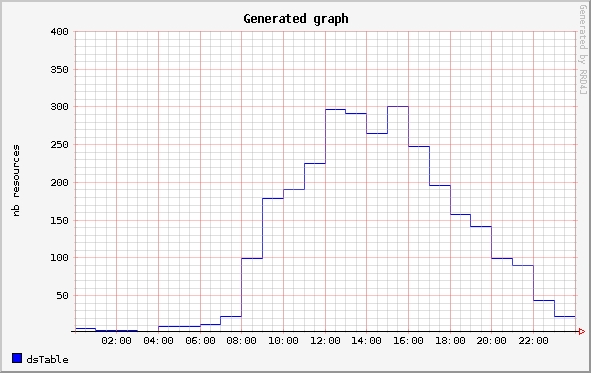
\includegraphics[scale=0.5]{exempleRRDtool.jpg}
	\caption{Exemple de graphe d'utilisation des salles informatiques de l'Universit\'e g\'en\'er\'e avec RRD4J}
	\label{figure:rrdTool}

\end{figure}

\subsection{Migration des donn\'ees}
\label{section:migrationDonnees}

Pendant le d\'eveloppement du projet, vue la quantit\'e de donn\'ees contenues dans la table \textsf{yuukou\_last} (environ 50 000 \`a 60 000 entr\'ees par mois), la question de l'archivage de ses donn\'ees s'est pos\'ee.
Une m\'ethode a donc \'et\'e recherch\'ee en consid\'erant le fait que les donn\'ees archiv\'ees peuvent \^etre r\'eutilis\'ees lors de l'ex\'ecution de quelques m\'ethodes par le client.

Une solution a \'et\'e trouv\'ee : le d\'eplacement \`a chaque d\'ebut de mois des donn\'ees dans une nouvelle table.
Chaque nouvelle table est identifi\'ee de la sorte : 

\begin{center}
	\textsf{yuukou\_last \_ ann\'ee mois}

\end{center}

Avec un exemple pour illustrer, \'etant en juin 2012, la table archiv\'ee correspondant au mois de mai portera le nom suivant : 

\begin{center}
	\textsf{yuukou\_last\_201205}

\end{center}

De cette mani\`ere, les donn\'ees contenues dans la table \textsf{yuukou\_last} correspondent aux mois en cours.

\subsection{L'acc\`es aux donn\'ees des tables}

Par souci de performance, \cad, limiter les acc\`es multiples \`a la base de donn\'ees mais aussi faciliter la manipulation des donn\'ees lors des traitements, le design pattern$^*$ \textit{Data Access Object} (DAO) a \'et\'e utilis\'e.
Un Data Access Object, ou objet d'acc\`es aux donn\'ees en fran\c{c}ais, est un objet qui constitue une repr\'esentation en m\'emoire des donn\'ees d'une base de donn\'ees.
En Java, un DAO est une classe repr\'esentant une table dont les attributs sont les champs de la table comme le montre la figure~\ref{figure:dao}.
Des classes repr\'esentant des listes sont g\'en\'eralement d\'evelopp\'e pour contenir les DAO et simplifier l'acc\`es aux donn\'ees.

Lorsqu'il sera n\'ecessaire d'effectuer des traitements r\'ep\'et\'es sur les donn\'ees d'une table, m\^eme si ces traitements ne portent pas sur la totali\'e de la table, il est pr\'ef\'erable de charger en m\'emoire la totalit\'e des \'el\'ements utiles avec, dans le cas id\'eal, une seule requ\^ete SQL$^*$.

\begin{figure}[!ht]
	\centering
	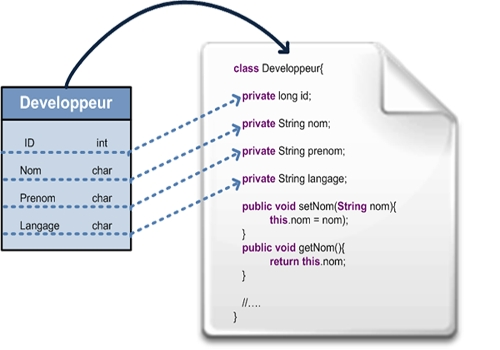
\includegraphics[scale=0.5]{dao.jpg}
	\caption{Exemple de \textit{mapping} d'une table avec sa classe DAO associ\'ee (\textit{source : Cyrille Herby})}
	\label{figure:dao}

\end{figure}

Dans le cadre du projet, les chargements sont effectu\'es lorsqu'un client appelle une m\'ethode du service Web. 
Les donn\'ees sont charg\'ees dans une liste, elles sont ensuite trait\'ees puis retourn\'ees au client.

\subsection{Le format de retour}
\label{section:formatRetour}

Le choix du type de retour est un choix important.
En effet, il faut que les donn\'ees puissent \^etre rapidement transmises, r\'ecup\'er\'ees, trait\'ees et affich\'ees.
L'objectif est un affichage instantan\'e des pages sur le navigateur Web ou l'application mobile.
De ce fait, plusieurs possibilit\'es ont \'et\'e envisag\'ees.


\subsubsection{{\og}\textit{Parsing}{\fg} d'un texte}

La premi\`ere est de transmettre un document texte basique, celui-ci format\'e d'une certaine fa\c{c}on afin d'\^etre \textit{pars\'e} ({\cad} parcourir un flux structur\'e d'informations pour en extraire les donn\'ees).
Ce qui aurait comme avantage de pouvoir \^etre r\'ecup\'er\'e par un client utilisant n'importe quel langage.
La figure~\ref{code:exemplePlaintext} repr\'esente une exemple de fichier qu'il est facile de \textit{parser}, il suffit de r\'ecup\'erer les informations se trouvant entre les arobases.

\vspace{0.20cm}

\begin{figure}[!ht]
	\begin{lstlisting}[language=plaintext]
	info1 @ info2 @ info3 @ info4
	\end{lstlisting}
	
	%\captionof{figure}{Exemple de ligne pouvant \^etre facilement \textit{pars\'ee}}
	\caption{Exemple de ligne pouvant \^etre facilement \textit{pars\'ee}}
	\label{code:exemplePlaintext}

\end{figure}

Pour r\'ecup\'erer les informations de cet exemple, il suffit de parcourir le fichier en stockant les informations contenues entre les \textbf{@}.

Cependant cette m\'ethode est assez contraignante et oblige \`a parcourir l'ensemble du fichier alors qu'un seul type d'information peut \^etre utile.
Ce qui signifie une perte de temps plus ou moins significative en fonction de la taille du fichier re\c{c}u.

\subsubsection{Objet Java s\'erialisable}

Une autre m\'ethode pourrait \^etre de transmettre un objet Java dit s\'erialisable.
La s\'erialisation est un m\'ecanisme fourni par Java permettant de consid\'erer un objet comme une s\'equence de d'octets qui inclut les donn\'ees de l'objet, le type de l'objet et le type des donn\'ees.
De cette mani\`ere, l'objet en question peut \^etre transmis \`a travers le r\'eseau vers une autre application Java pour le r\'ecup\'erer et le d\'es\'erialiser, ce qui repr\'esente la proc\'edure inverse de la s\'erialisation.
La figure~\ref{code:exempleJava} donne un exemple de classe Java s\'erialisable qui pourrait \^etre transmise par le r\'eseau comme un flux de bytes.

\vspace{0.20cm}

\begin{figure}[!ht]
	\lstinputlisting[language=Java]{codes/Exemple.java}
	%\captionof{figure}{Exemple de classe Java s\'erialisable}
	\caption{Exemple de classe Java s\'erialisable}
	\label{code:exempleJava}

\end{figure}

L'objet contiendrait toutes les donn\'ees utiles et celles-ci seraient facilement accessibles.
Le probl\`eme venant avec cette solution est que les objets doivent \^etre r\'ecup\'er\'es par une JVM$^*$.
Ce qui peut s'av\'erer plus ou moins compliqu\'e voir impossible dans d'autres langages de programmation que Java.

\subsubsection{XML}

eXtensible Markup Language ou XML est un m\'eta langage pour r\'ealiser du balisage g\'en\'erique permettant de mettre en forme les documents. XML a connu un grand succ\`es depuis sa cr\'eation.
Il est utilis\'e en particulier pour g\'erer la configuration, le stockage des donn\'ees, l'\'echange d'informations et bien d'autres fonctions encore.
La figure~\ref{code:exempleXML} donne un exemple de document XML pouvant \^etre facilement converti en une arborescence DOM$^*$.

\vspace{0.20cm}

\begin{figure}[!ht]
	\lstinputlisting[language=XML]{codes/Exemple.xml}
	%\captionof{figure}{Exemple de document XML}
	\caption{Exemple de document XML}
	\label{code:exempleXML}

\end{figure}

XML offre une solution structur\'ee et tr\`es simple \`a comprendre pour l'envoi d'information par le r\'eseau, cependant dans les \'echanges d'informations entre client et serveur, il montre ses limites :

\begin{itemize}
	\item le chargement et la manipulation deviennent vite compliqu\'es, la plupart du temps il est n\'ecessaire de \textit{parser} le XML sous forme de DOM$^*$, puis de le parcourir, ce qui requiert l'appel de nombreuses fonctions, sans mentionner le fait que \textit{parser} un document XML est parfois long;
	\item la taille des fichiers \'echang\'es peut parfois \^etre cons\'equente du fait de la duplication des donn\'ees : par nature, le XML ne permet pas de g\'erer une \'enorme masse d'informations.

\end{itemize}

\subsubsection{JSON}

JavaScript Object Notation ou JSON est un format l\'eger d'\'echange de donn\'ees texte.
Il utilise la notation des objets JavaScript pour transmettre de l'information structur\'ee.
Il est aussi souvent utili\'e pour simplifier et all\'eger les acc\`es \`a des services Web depuis les navigateurs.
La figure~\ref{code:exempleJSON} donne une exemple de fichier JSON reprenant le m\^eme arbre que le document XML de la figure~\ref{code:exempleXML}.

\vspace{0.20cm}

\begin{figure}[!ht]
	\lstinputlisting[language=JSON]{codes/Exemple.json}
	%\captionof{figure}{Exemple de fichier JSON}
	\caption{Exemple de fichier JSON}
	\label{code:exempleJSON}

\end{figure}

\subsubsection{Choix du format}

Le choix du format de retour des donn\'ees s'est port\'e sur l'utilisation de JSON.
Le but du client, qui demande des informations au service Web, est de recevoir les donn\'ees le plus rapidement possible afin d'avoir \`a les afficher dans la foul\'ee.
De ce fait, le \textit{parsing} d'un texte contenant des balises \`a certains endroits s'av\`ere inadapt\'e, notamment pour r\'ecup\'erer un seul type d'information.
L'envoi d'un objet s\'erialisable Java est, quant \`a lui trop restrictif. Le choix a donc \'et\'e de choisir entre XML ou JSON.

XML offre un format de donn\'ees verbeux et prend beaucoup d'espace. 
De plus un document XML peut \^etre valid\'e via l'utilisation de DTD\protect\footnote{\textit{Document Type Definition}}, document permettant de d\'ecrire un mod\`ele de document XML, ou de XSD\protect\footnote{\textit{XML Schema Definition}}, langage de description de format de document XML permettant de d\'efinir la structure et le type de contenu d'un document XML.

JSON offre un format de fichier plus simple que XML, facilement compr\'ehensible.
Pour compl\'eter, les fichiers JSON, \`a arbre \'egal, seront toujours plus petits que l'\'equivalent XML et pr\'esenteront l'avantage d'\^etre plus rapidement \textit{pars\'es}.

Au final JSON permet une plus grande rapidit\'e dans les \'echanges avec un serveur ainsi que sur le temps de \textit{parsing} des fichiers, le tout avec une \'economie des ressources du fait de sa petit taille.
Cependant, les donn\'ees ne peuvent pas \^etre v\'erifi\'ees dans un fichier JSON, il demande donc une certaine rigueur dans son \'ecriture du cot\'e serveur ainsi qu'une connaissance de sa structure du cot\'e client.

\subsection{Compl\'ement d'information sur JSON}

\subsubsection{Pr\'esentation}

Une courte description de ce qu'est JSON a d\'ej\`a \'et\'e faite au \S~\ref{section:formatRetour}.
Pour reprendre ce qui a d\'ej\`a \'et\'e dit, JSON est un format l\'eger d'\'echange de donn\'ees qui est apparu en 2002.
Il est facile \`a \'ecrire et comprendre pour des humains.
Il est bas\'e sur un sous-ensemble du langage de programmation JavaScript et est compl\`etement ind\'ependant de tout langage, tout en poss\`edant des conventions famili\`eres aux langages descendant du C (C++, C\#, Java, JavaScript, \ldots).
Ces propri\'et\'es font de JSON un langage d'\'echange de donn\'ees id\'eal.

Cependant, il ne supporte pas les espaces de noms au contraire d'XML.
Pour la v\'erification des donn\'ees, les sch\'emas JSON ne sont pas tr\`es utilis\'es du fait qu'ils doivent \^etre ecrit \`a la main comme il n'existe aucun outil pour g\'en\'erer un sch\'ema \`a partir de donn\'ees JSON.
Et concernant la s\'ecurit\'e, il existe la possibilit\'e o\`u des \textit{scripts} malveillants pourraient \^etre dissimul\'es et ex\'ecut\'es.
Il existe des fonctions pour tester les fichiers JSON mais celles-ci ne sont pas vraiment concluantes.
La meilleure d\'efense est de conna\^itre \`a l'avance les points sensibles et de prendre les pr\'ecautions n\'ecessaires.

\subsubsection{Structure}

JSON se base sur deux structures de donn\'ees universelles dans pratiquement tous les langages de programmation modernes :

\begin{itemize}
	\item une collection de couples nom/valeur;
	\item une liste de valeurs ordonn\'ees.

\end{itemize}

\vspace{0.20cm}

\noindent Ces \'el\'ements repr\'esentent trois types de donn\'ees :

\begin{itemize}
	\item un \textit{objet} :\\Ensemble de couples nom/valeur non ordonn\'es. Un objet commence par \textsf{\{ (accolade gauche)} et se termine par \textsf{\} (accolade droite)}.
	Chaque nom est suivi de \textsf{: (deux-points)} et les couples nom/valeur sont s\'epar\'es par \textsf{, (virgule)};
	\item un \textit{tableau} :\\Collection de valeurs ordonn\'ees. Un tableau commence par \textsf{$[$ (crochet gauche)} et se termine par \textsf{$]$ (crochet droit)}.
	Les valeurs sont s\'epar\'ees par \textsf{, (virgule)};
	\item une \textit{valeur} :\\Soit une \textsf{cha\^ine de caract\`eres} entre guillemets, soit un \textsf{nombre}, soit \textsf{true} ou \textsf{false} ou \textsf{null}, soit un \textsf{objet}, soit un \textsf{tableau}.
	Ces structures peuvent \^etre imbriqu\'ees;
	\item une \textit{cha\^ine de caract\`eres} :\\Suite caract\'eres Unicode (z\'ero ou plus), entre guillemets, et utilisant les \'echappements avec antislash. 
	Un caract\`eres est repr\'esent\'e par une cha\^ine d'un seul caract\`ere.

\end{itemize}

\subsection{Gestion de la base de donn\'ees}

La base de donn\'ees a \'evolu\'e tout au long du projet en fonction des fonctionnalit\'es qui ont \'et\'e demand\'ees.
L'annexe~\ref{chapterAnnexe:baseDeDonnees} permet d'avoir une description des diff\'erentes tables composant la base de donn\'ees, une vue g\'en\'erale de ce \`a quoi elle ressemble, et des vues d\'ecoup\'ees des diff\'erentes parties.

La base de donn\'ees peut \^etre d\'ecoup\'ee en diff\'erentes grandes parties.
La partie archivage a pour but de conserver les donn\'ees dans le temps.
Pour ce faire, elle est compos\'ee de deux tables centrales de sauvegarde d'informations.
La premi\`ere est la table \textsf{yuukou\_who}, son but est de simuler la commande UNIX \textsf{who}.
Cette commande permet de donner tous les utilisateur connect\'es sur la machine o\`u elle est ex\'ecut\'ee.
De ce fait, si elle est port\'ee au niveau de Nagios et du projet, la table contiendra tous les utilisateurs connect\'es sur un ordinateur et depuis quand ils le sont.
La deuxi\`eme table est \textsf{yuukou\_last}, son but est aussi de simuler une commande UNIX, la commande \textsf{last}.
Cette commande permet de donner la liste de toutes les derni\`eres connexions sur la machine sur laquelle elle est ex\'ecut\'ee.
De ce fait, si elle est port\'ee au niveau de Nagios et du projet, la table contiendra toutes les connexions des utilisateurs sur un ordinateur, l'heure de d\'ebut et de fin et la cause de la d\'econnexion. En fait, elle contiendra les donn\'ees de la table \textsf{yuukou\_who} et ajoutant les informations du temps de fin de connexion et la cause de la d\'econnexion.

La partie logicielle a pour but de stocker la configuration logicielle de chaque salle informatique.
La r\'ecup\'eration de cette configuration est expliqu\'ee au \S~\ref{section:catalogueLogiciel}.
Cette partie est compos\'ee de plusieurs tables.
Une salle informatique peut avoir des groupes de logiciels, \textsf{yuukou\_rooms\_groups} et aussi des logiciels ind\'ependants de tout groupe, \textsf{yuukou\_rooms\_software}.
Un groupe de logiciels contient des logiciels, \textsf{yuukou\_groups\_software}.
Les descriptions des groupes et logiciels sont contenues dans les tables \textsf{yuukou\_groups} et \textsf{yuukou\_software}.
Avec ces tables, il est possible de facilement reconstruire la configuration logicielle d'une salle.

La partie emploi du temps a pour but de stocker tous \'ev\`enements des diff\'erents emplois du temps de l'Universit\'e.
La r\'ecup\'eration de cette configuration est expliqu\'ee au \S~\ref{section:emploiDuTemps}.
Cette partie est compos\'ees de trois tables.
La premi\`ere table est celle contenant toutes les salles \textsf{yuukou\_rooms}, la deuxi\`eme contenant tous les \'ev\`enements \textsf{yuukou\_timetables}.
Pour la derni\`ere table \textsf{yuukou\_mapping\_room}, son r\^ole est de faire le lien entre les noms des salles dans Nagios et les noms des salles qui sont utilis\'ees pour l'emploi du temps.
En effet, la g\'en\'eration des emplois du temps est effectu\'ee par un service de l'Universit\'e.
De ce fait, ce service utilise un syst\`eme pour nommer les salles qui lui est propre.
Il est donc n\'ecessaire de pouvoir relier un \'ev\`enement \`a une salle \`a l'aide de cette derni\`ere table.

La partie \textit{mapping} avec les salles a pour but de faire le lien entre une description compl\`ete d'un lieu et la description courte qui est donn\'e dans la description d'une salle dans la table \textsf{yuukou\_rooms}.
Les informations concernant les diff\'erents lieux sont contenues dans la table \textit{yuukou\_mapping\_location}.

La derni\`ere partie, configuration, a pour but de g\'erer les diff\'erents param\`etres permettant la gestion de cycle lors du fonctionnement du service Web. 
Les explications concernant ce qu'est un cycle se trouvent au \S~\ref{section:cyclePrincipal}.

TODO a finir

\section{Organisation du travail}

\subsection{Gestion du poste de travail}
\label{section:gestionProjet}

Afin de d\'evelopper efficacement, une organisation du poste de travail mais plus g\'en\'eralement du projet en lui-m\^eme a \'et\'e choisie.
Cette organisation comporte une machine de d\'eveloppement et deux serveurs comme le montre la figure~\ref{figure:gestionProjet}.

\begin{figure}[!ht]
	\centering
	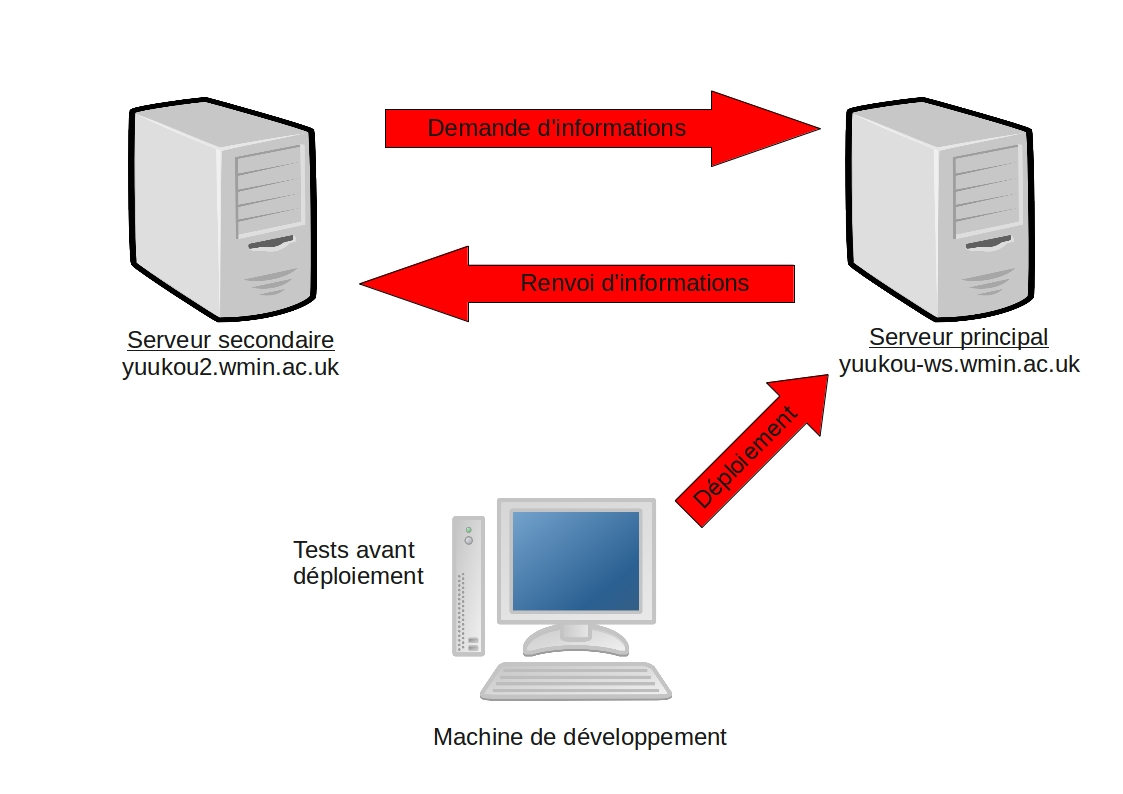
\includegraphics[scale=0.35]{gestionProjet.jpg}
	\caption{Sch\'ema de la gestion du projet}
	\label{figure:gestionProjet}

\end{figure}

Le serveur principal poss\`ede un syst\`eme d'exploitation Debian version 6.0.5 (\textit{Squeeze}) et h\'eberge le service Web dans une version stable ainsi que tous les outils n\'ecessaire \`a son fonctionnement comme le serveur de gestion de base de donn\'ees (SGBD) MySQL, une version de Java \`a jour, le serveur d'application GlassFish mais aussi Nagios.
La faible consommation CPU de Nagios dans la surveillance des machines de l'universit\'e fait, qu'actuellement, il peut \^etre h\'eberg\'e sur le m\^eme serveur que le service Web.
Le serveur principal h\'eberge aussi le gestionnaire de version subversion (SVN) sur lequel est constamment maintenu le projet.
Il est accessible sur le r\'eseau sous le nom de domaine \textsf{yuukou-ws.wmin.ac.uk}.

Le serveur dit {\og}secondaire{\fg} poss\`ede lui aussi le m\^eme syst\`eme d'exploitation Debian et h\'eberge l'application Web permettant de communiquer avec le service Web.
Cette application fait r\'eguli\`erement appel au service Web pour obtenir les informations dont elle a besoin pour afficher correctement ses pages.
Il est accessible sur le r\'eseau sous le nom de domaine \textsf{yuukou2.wmin.ac.uk}.

La machine de d\'eveloppement poss\`ede un syst\`eme d'exploitation Linux Mint version 11 (\textit{Katya}), tous les outils n\'ecessaires au d\'eveloppement (comme Java, NetBeans, \ldots), mais aussi un serveur de gestion de base de donn\'ee (SGBD) MySQL et un serveur GlassFish, tous deux servant \`a effectuer des tests avant d\'eploiement.
\`A chaque d\'eploiement sur le serveur principal, la version du projet est publi\'ee sur le SVN afin de garantir une s\'ecurit\'e dans le cas d'une r\'egression dans le d\'eveloppement.

\subsection{Travail en \'equipe}

Le projet {\YuukouII}, comme \'enonc\'e dans le \S~\ref{section:architectureProjet}, a \'et\'e divis\'e en deux parties.
La partie service Web, permettant de remplir et maintenir la base de donn\'ees ainsi que de mettre \`a disposition d'un client des m\'ethodes retournant une partie des informations r\'ecup\'er\'ees, et la partie affichage dont le r\^ole est de pr\'esenter les informations \`a un utilisateur lambda.
La partie affichage fut confi\'ee \`a Yacine MAGHEZZI, \'etudiant en 3\up{i\`eme} ann\'ee de licence informatique \`a l'Universit\'e de Franche-Comt\'e de Besan\c{c}on.
Le but de son projet \'etait, \`a l'aide du service Web, de permettre un affichage r\'esumant la disponibilit\'e des laboratoires informatiques dans l'Universit\'e.

Ainsi, \`a chaque red\'eploiement du service Web lors d'une mise \`a jour importante ou d'un ajout de fonctionnalit\'es, il \'etait important de le tenir inform\'e des diff\'erents changements qui ont \'et\'e effectu\'es.
TODO : reference structure
C'est dans le cadre de ce travail en \'equipe qu'une structure de retour standard a \'et\'e adopt\'ee.
En effet, un minimum de rigueur dans le d\'eveloppement permettait de ne pas avoir de surprises \`a chaque \'etape du projet.

Cependant, la majeure partie de la communication se faisait selon les besoins de M. MAGHEZZI.
Avant son arriv\'ee, les fonctionnalit\'es et les informations qu'elles retournaient n'\`etaient que limit\'ees.
Cela \'etant d\^u au fait que les informations retourn\'ees n'\'etaient exploit\'ees par personne.
Apr\`es son arriv\'ee et sa premi\`ere connexion au service Web, M. MAGHEZZI a commenc\'e \`a exprimer des demandes concernant les \'el\'ements qu'il aimerait voir appara\^itre.
C'est \`a ce moment que le dialogue s'est vraiment mis en place.

\'Etant dans le m\^eme bureau, la communication se d\'eroulait principalement oralement, il \'etait inform\'e directement et m\^eme en avance par rapport au d\'eploiement d'une nouvelle version du service Web.
Concernant les structures de retour JSON, il arrivait qu'un mail lui soit envoy\'e, ce mail contenant le sch\'ema d'une structure de retour de tous les cas possibles pour une m\'ethode sp\'ecifique du service Web.

\subsection{Tests du service Web}

\subsubsection{Mise en place d'un client}

\subsubsection{Consommation les m\'ethodes}


\section{Probl\`emes rencontr\'es}

Durant toute la dur\'ee du projet, de nombreux probl\`emes ont \'et\'e rencontr\'es.
Ils \'etaient principalement dus au manque de connaissances dans le domaine vis\'e.

Le SSL\protect\footnote{\textit{Secure Sockets Layer}} a \'et\'e difficilement mis en place dans les premiers temps.
En effet, le manque de connaissance dans les services Web et dans les outils NetBeans et GlassFish ont \'et\'e un frein dans sa mise en place.
De plus, la documentation sur le Web est plus ou moins \'evasive et les m\'ethodes sont diverses pour s\'ecuriser un service Web.
Cependant, avec l'aide de l'Universit\'e, notamment en fournissant les diff\'erents certificats et les instructions, le protocole a pu \^etre mis en fonction.

Il est apparu pendant le stage que les diff\'erents services de l'Universit\'e n'appliquaient que rarement les m\^emes normes.
Cela s'est fait ressentir dans la mise en place de la gestion des emplois du temps.
Effectivement, les noms des salles entre {\YuukouII} et ceux dans les emplois du temps n'avaient rien \`a voir.
Certes, certaines pouvaient \^etre devin\'ees, elles ont \'et\'e de ce fait trait\'ees.
Mais pour d'autres cela s'av\'erait impossible, surtout si on consid\`ere que plusieurs personnes s'occupent des emplois du temps et que ces personnes appliquent chacun une m\'ethode de nommage plus ou moins diff\'erentes les unes des autres.
Une r\'eunion a eu lieu pendant le stage avec l\'equipe en charge afin d'aborder ce point.
Au final, un nouveau syst\`eme d'identification des salles devrait \^etre mis en place, mais le service \'etant occup\'e, il n'y a pas de date dans la mise en fonction d'une telle mesure.
Lorsque ce syst\`eme sera appliqu\'e, la liste des nouveaux noms de salles sera communiqu\'ee, ce qui rendra cette partie pleinement fonctionnelle.

TODO a finir



\clearpage
